% ----
% COMP1204 CW1 Report Document
% ----
\documentclass[]{article}

% Reduce the margin size, as they're quite big by default
\usepackage[margin=1in]{geometry}

%Importing fancy package
\usepackage{fancyvrb}
\usepackage[most]{tcolorbox}
\usepackage{xcolor}
\usepackage{graphicx}
\graphicspath{ {./images/} }
\usepackage{blindtext}
\usepackage{soul}
\usepackage[T1]{fontenc}

\title{COMP1204: Data Management \\ Coursework One: Hurricane Monitoring }
% Update these!
\author{Damien Ta \\ 34830294}

% Actually start the report content
\begin{document}

% Add title, author and date info
\maketitle

\section{Introduction}
As data scientists for the National Oceanographic and Atmospheric Administraiton Centre, I was assigned to the tropical cyclone
tracking team. As a data scientist I have been tasked with extracting storm data from the tropical cyclone reports and producing
maps of where the cyclones have taken place.
\section{Create CSV Script}
Here's my script:
\begin{tcolorbox}[colback=white, colframe=black, boxrule=0.5pt, arc=2mm, 
    title=create\_csv.sh, fonttitle=\bfseries, listing only, listing options={language=sh, basicstyle=\ttfamily}]
    \begin{verbatim}
#!/bin/bash
csv_input_path=$1
tmp_csv_output=$2

echo "Timestamp,Latitude,Longitude,MinSeaLevelPressure,MaxIntensity" > $tmp_csv_output
dtg="$(grep -R "<dtg>" $csv_input_path | sed 's/.*<dtg>//g' | sed 's/[</dtg>]//g')"
grep -R "<lat>" $csv_input_path| sed 's/.*<lat>//g' | sed 's/[</lat>]//g' > lat.csv
grep -R "<lon>" $csv_input_path | sed 's/.*<lon>//g' | sed 's/[</lon>]//g' > lon.csv
grep -R "<minSeaLevelPres>" $csv_input_path | sed 's/.*<minSeaLevelPres>//g' | /
sed 's/[</minSeaLevelPres>]//g' > minSeaLevelPres.csv
grep -R "<intensity>" $csv_input_path | sed 's/.*<intensity>//g' | / 
sed 's/[</intensity>]//g' > intensity.csv

lat="$(sed "s/$/ N/" lat.csv)"
lon="$(sed "s/$/ W/" lon.csv)"
minSeaLevelPres="$(sed "s/$/ mb/" minSeaLevelPres.csv)"
maxIntensity="$(sed "s/$/ knots/" intensity.csv)"

paste -d',' <(echo "$dtg") <(echo "$lat") <(echo "$lon") <(echo "$minSeaLevelPres") \
<(echo "$maxIntensity") >> $tmp_csv_output

rm lat.csv
rm lon.csv
rm minSeaLevelPres.csv
rm intensity.csv

#I used / to continue command on next line
    \end{verbatim}
\end{tcolorbox}
I will now explain my code in small boxes each in its own independent sections:
\begin{tcolorbox}[colback=white, colframe=black, boxrule=0.5pt, arc=2mm, 
    title=First part of the code, fonttitle=\bfseries, listing only, listing options={language=sh, basicstyle=\ttfamily}]

    \begin{verbatim}
#!/bin/bash
csv_input_path=$1
tmp_csv_output=$2
    \end{verbatim}
\hl{\#\!/bin/bash}\newline
tells the terminal that when you run the script it should use bash to execute it\newline
\hl{csv\_input\_path=\$1}\newline
\hl{tmp\_csv\_output=\$2}\newline
These two lines of code allow inputs to be enntered into the script
\end{tcolorbox}
\begin{tcolorbox}[colback=white, colframe=black, boxrule=0.5pt, arc=2mm, 
    title=Second part of the code, width=6.7in, fonttitle=\bfseries, listing only, listing options={language=sh, basicstyle=\ttfamily}]
    \begin{verbatim}
1 echo "Timestamp,Latitude,Longitude,MinSeaLevelPressure,MaxIntensity" > $tmp_csv_output
2 dtg="$(grep -R "<dtg>" $csv_input_path | sed 's/.*<dtg>//g' | sed 's/[</dtg>]//g')"
3 grep -R "<lat>" $csv_input_path| sed 's/.*<lat>//g' | sed 's/[</lat>]//g' > lat.csv
4 grep -R "<lon>" $csv_input_path | sed 's/.*<lon>//g' | sed 's/[</lon>]//g' > lon.csv
5 grep -R "<minSeaLevelPres>" $csv_input_path | sed 's/.*<minSeaLevelPres>//g' | \
6 sed 's/[</minSeaLevelPres>]//g' > minSeaLevelPres.csv
7 grep -R "<intensity>" $csv_input_path | sed 's/.*<intensity>//g' | \ 
8 sed 's/[</intensity>]//g' > intensity.csv
    \end{verbatim}
\hl{echo "Timestamp,Latitude,Longitude,MinSeaLevelPressure,MaxIntensity" > \$tmp\_csv\_output}\newline
This command prints the tag headers\newline
\hl{dtg="\$(grep -R "<dtg>" \$csv\_input\_path | sed 's/.*<dtg>//g' | sed 's/[</dtg>]//g')"}\newline
The code creates variable dtg, we grep the kml file inputted at \$1 and search recursively for\newline
keyword <dtg>. The sed 's/.*<dtg>//g' command would replace any character and its occurences \newline
with an empty space including anything before the pattern.\newline
the sed 's/[</dtg>]//g' command would replace any characters between the [], so < / d t g >\newline
to an empty character and the g stands for global.\newline
\hl{grep -R "<lat>" \$csv\_input\_path | sed 's/.*<lat>//g' | sed 's/[</lat>]//g' > lat.csv}\newline
grep recursively keyword <lat> from the kml file inputted\newline
The sed 's/.*<dtg>//g' command would replace any character and its occurences \newline
with an empty space including anything before the pattern.\newline
The sed 's/[</lat>]//g' command would replace any characters between the [ ], so < / l a t >\newline
The outcome is then appended to a file called lat.csv for later use. This same code is then run\newline
on the rest of the tag headers Longitude, MinSeaLevelPressure and MaxIntensity.\newline


\end{tcolorbox}

\begin{tcolorbox}[colback=white, colframe=black, boxrule=0.5pt, arc=2mm, 
    title=Third part of the code, fonttitle=\bfseries, listing only, listing options={language=sh, basicstyle=\ttfamily}]
    \begin{verbatim}
lat="$(sed "s/$/ N/" lat.csv)"
lon="$(sed "s/$/ W/" lon.csv)"
minSeaLevelPres="$(sed "s/$/ mb/" minSeaLevelPres.csv)"
maxIntensity="$(sed "s/$/ knots/" intensity.csv)"
    \end{verbatim}
    \hl{lat="$(sed "s/$/ N/" lat.csv)"}\newline
    New variable lat is created which uses sed and adds on each line (\$) " N" from file lat.csv\newline
    This is then run on each line of code for longitude, minSeaLevelPres and maxIntensity for their\newline
    respective unit of measure.\newline
    \hl{lon="$(sed "s/$/ W/" lon.csv)"}\newline
    \hl{minSeaLevelPres="$(sed "s/$/ mb/" minSeaLevelPres.csv)"}\newline
    \hl{maxIntensity="$(sed "s/$/ knots/" intensity.csv)"}\newline
\end{tcolorbox}
\clearpage



\section{Storm Plots}
\subsection{Storm Plot 1}
\begin{figure}[htbp]
    \centering
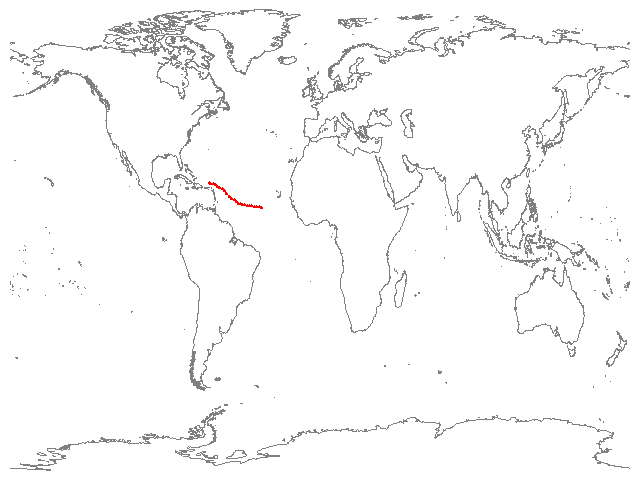
\includegraphics{al112020.png}
\caption{al112020.kml}
\label{fig:al112020}
\end{figure}

\clearpage
\subsection{Storm Plot 2}

\begin{figure}[htbp]
    \centering
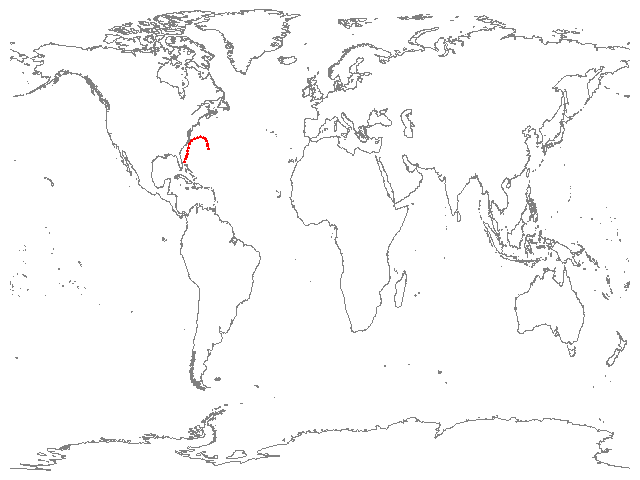
\includegraphics{al012020.png}
\caption{al012020.kml}
\label{fig:al012020}
\end{figure}

\clearpage
\subsection{Storm Plot 3}

\begin{figure}[htbp]
    \centering
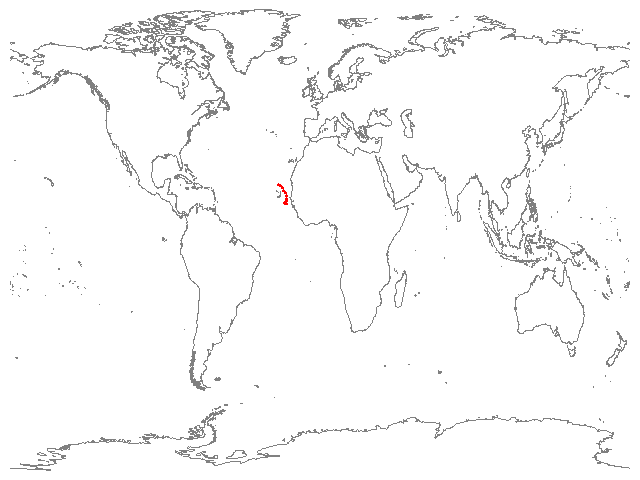
\includegraphics{al102020.png}
\caption{al102020.kml}
\label{fig:al102020}
\end{figure}
\clearpage
\section{Git Usage}
\begin{tcolorbox}[enhanced, 
    listing only,
    title=Python Code for Plotting CSV Data,
    fonttitle=\bfseries,
    colback=white,
    colframe=black!70,
    listing options={
      language=Python,
      numbers=left, 
      numberstyle=\tiny\color{gray},
      breaklines=true, 
      basicstyle=\ttfamily\small, 
      columns=fullflexible,
      keepspaces=true,
      showstringspaces=true,
    },]
    \begin{verbatim}
        import pandas as pd
        import matplotlib.pyplot as plt
        import os
        import glob
        import math
        user_key = 1773
        
        def plot_all_csv_pressure():
            path = os.getcwd()
            csv_files = glob.glob(os.path.join(path, '*.csv'))
            
            for f in csv_files:
                storm = pd.read_csv(f)
                storm['Pressure'].plot()
                plt.show()
        
        def plot_all_csv_intensity():
            path = os.getcwd()
            csv_files = glob.glob(os.path.join(path, '*.csv'))
            
            for f in csv_files:
                storm = pd.read_csv(f)
                storm['Intensity'].plot()
                plt.show()
    \end{verbatim}
\end{tcolorbox}


\end{document}
